\chapter{Context}
TODO what's this thesis about (general scope)

\section{Initial Situation}
TODO What's Roadster and its goals

\section{Software Architecture}
TODO Roadster architecture\\

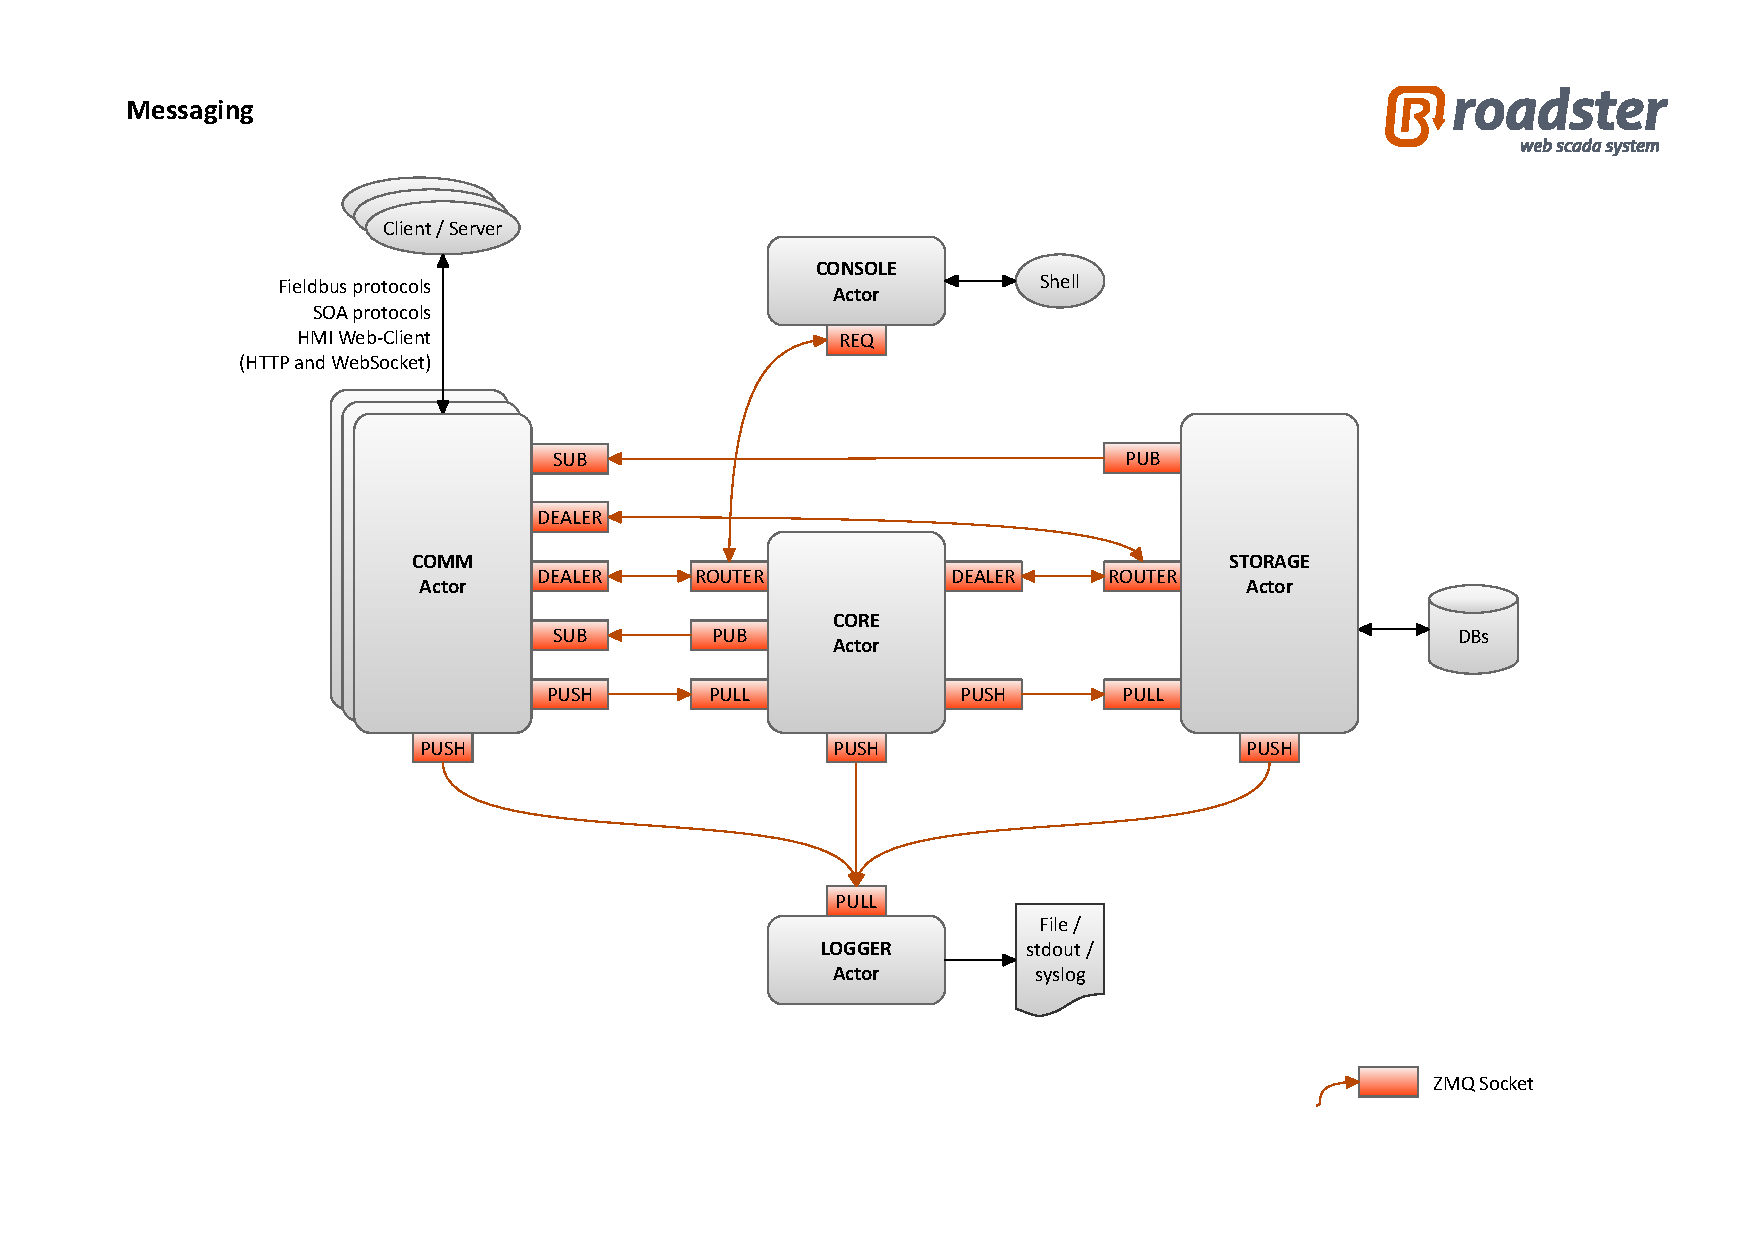
\includegraphics[trim=4cm 2cm 3.5cm 2.8cm, clip=true, width=\textwidth]{img/roadster_arch.pdf}

\section{Goals}
TODO mandatory goals

\subsection*{Optional Goals}
TODO optional goals

\section{Requirements}
TODO the requirements

In descending priority:

\begin{enumerate}
\item multi-node CSP
\item single-level HA
\item multi-level HA
\item persistence synchronization
\item security
\item OPC UA HA (optional)
\end{enumerate}

The following sections explain the requirements in greater detail.

\subsection{Cluster}
This could also be called "Multi-node CSP".

\begin{itemize}
\item this is to allow running Roadster in a hierarchical setup
\item new COMM actors for inter node communication
\item usually 2 (or 3) levels of Roadster nodes
\item common cases:
\begin{itemize}
\item   - single level, single node (legacy)
\item   - single level HA
\item   - multi level, HA at root node only
\end{itemize}
\item exotic cases:
\begin{itemize}
\item   - multi level, HA at bottom
\item   - multi level, HA in middle
\end{itemize}
\item every subtree can live on autonomously
\item only node A has write access to values on A (to avoid uncertain situations involving race conditions), e.g.:
\begin{itemize}
\item - a forced value coming from the web UI comes through a command,
\item - routed to the relevant node, where it is applied,
\item - and then synced (up via DEALER and down via PUB, we suppose)
\end{itemize}
\item KISS
\end{itemize}


\begin{lstlisting}[style=customsh]
       C
     /   \
    A     B
\end{lstlisting}



\subsection{Single Level HA}
This is where there's a node pair directly connected to a PLC. Both nodes have read/write access to the PLC, but only one of the nodes (the active one) must do so. The nodes must automatically find consensus on who's active. The passive one must automatically take over in case the active one is confirmed to be dead.



\subsection{Multi Level HA}
This is where a node pair is the parent of one or more other nodes (subnodes).

\subsection{Persistence Synchronization}
This is about the synchronization of the TokyoCabinet databases. Data flow is from south to north (towards the root node), so the root node collects and maintains a replication of the persisted data of all subnodes, recursively.

\begin{itemize}
	\item autonomous
	\item not same as CHP
	\item data only flows from bottom to top
\end{itemize}

\subsection{Security}
\begin{itemize}
	\item transport needs to be secure (encrypted and authenticated)
	\item TODO verify requirements with Andy (we didn't really discuss this during the meeting)
\end{itemize}

\subsection{OPC UA HA}
\begin{itemize}
	\item provide standardized interface upwards from HA pairs
\end{itemize}

% ---------------------------------------------------------------------------
\subsection{Non-Functional Requirements}
TODO the NFRs

\subsubsection{Coding Guidelines}
\begin{itemize}
	\item basically Ruby style guide\footnote{\url{https://github.com/bbatsov/ruby-style-guide}}
	\item method calls: only use parenthesis when needed, even with arguments (as opposed to \footnote{\url{https://github.com/bbatsov/ruby-style-guide\#method-invocation-parens}})
	\item 2 blank lines before method definition (slightly extending \footnote{\url{https://github.com/bbatsov/ruby-style-guide\#empty-lines-between-methods}})
	\item YARD API doc, 1 blank comment line before param documentation, one blank comment line before code (ignoring \footnote{\url{https://github.com/bbatsov/ruby-style-guide\#rdoc-conventions}})
	\item Ruby 1.9 symbol keys are wanted (just like \footnote{\url{https://github.com/bbatsov/ruby-style-guide\#hash-literals}})
	\item align multiple assignments so there's a column of equal signs
\end{itemize}


\section{Task Description}
TODO our tasks

